\chapter{Licht en schaduw}\label{ch:g1:light-and-shadows}

Doe de lamp uit in een kamer zonder raam: alles verdwijnt. Doe hem
aan: de kamer komt terug. Zien heeft \omterm{def:g1:light-and-shadows:source}{licht} nodig. En overal waar
\omterm{def:g1:light-and-shadows:source}{licht} is, is ook \omterm{def:g1:light-and-shadows:shadow}{schaduw} --- je trouwe donkere tweelingbroer
volgt je op elke zonnige stoep. Laten we uitzoeken waar \omterm{def:g1:light-and-shadows:source}{licht}
vandaan komt, en hoe \omterm{def:g1:light-and-shadows:shadow}{schaduwen} ontstaan.

\section{Waar licht vandaan komt}

\begin{definition}[Lichtbronnen]\label{def:g1:light-and-shadows:source}
Een \emph{lichtbron}\index{lichtbron} is iets dat zijn eigen
\emph{licht}\index{licht} maakt: de Zon, een lamp, een kaarsvlam, een
glimworm. Al het andere --- een boek, een bal, de muren, jij --- maakt
geen eigen licht: we zien die dingen alleen als er licht van een bron
op valt.
\end{definition}

\begin{example}[Bron of geen bron?]\label{ex:g1:light-and-shadows:sources}
De Zon, een zaklamp, een brandende lucifer en een televisiescherm
maken allemaal \omterm{def:g1:light-and-shadows:source}{licht}: bronnen. De Maan, een spiegel en een witte muur
kunnen er heel helder uitzien, maar ze maken geen eigen
\omterm{def:g1:light-and-shadows:source}{licht} --- ze sturen alleen \omterm{def:g1:light-and-shadows:source}{licht} terug dat hen bereikt. Doe de lamp
uit, en de helderste spiegel wordt donker.
\end{example}

\begin{example}[Probeer het: de donkere kamer]\label{ex:g1:light-and-shadows:darkroom}
Sluit 's avonds de luiken of de gordijnen van een kamer, doe alle
lampen uit en wacht terwijl je rustig tot $20$ telt. Wat zie je? Eerst
bijna niets --- zonder bron is er geen \omterm{def:g1:light-and-shadows:source}{licht} om bij te zien. Zet dan
de deur op een kier: één dun reepje \omterm{def:g1:light-and-shadows:source}{licht} is genoeg om tafels,
stoelen en speelgoed terug te brengen.
\end{example}

\begin{remark}[Kijk nooit in de Zon]\label{rem:g1:light-and-shadows:sun}
De Zon is verreweg de sterkste \omterm{def:g1:light-and-shadows:source}{lichtbron} die we ooit tegenkomen. Kijk
er nooit recht in, zelfs niet heel even, en al helemaal niet door een
verrekijker of een vergrootglas: haar \omterm{def:g1:light-and-shadows:source}{licht} is zo sterk dat het je
ogen voorgoed kan beschadigen. Van de Zon geniet je zijdelings ---
via het \omterm{def:g1:light-and-shadows:source}{licht} dat ze op alles om je heen werpt.
\end{remark}

\section{Hoe schaduwen ontstaan}

\begin{definition}[Schaduw]\label{def:g1:light-and-shadows:shadow}
Een \emph{schaduw}\index{schaduw} is de donkere plek die verschijnt
achter een ding dat het \omterm{def:g1:light-and-shadows:source}{licht} tegenhoudt. \omterm{def:g1:light-and-shadows:source}{Licht} kan niet door je
lichaam heen, dus achter jou krijgt de grond geen \omterm{def:g1:light-and-shadows:source}{licht} van de Zon:
die donkere plek in jouw vorm is jouw schaduw.
\end{definition}

\begin{omfigure}
\begin{tikzpicture}[scale=0.85]
  % two rays from the lamp, exactly tangent to the ball (computed:
  % source (0,1.5), ball center (4.2,1.5), r=0.55 -> wall hits y=1.5±1.004)
  \draw[omThm] (0,1.5) -- (7.6,2.504);
  \draw[omThm] (0,1.5) -- (7.6,0.496);
  % free rays that miss the ball entirely
  \draw[omThm] (0,1.5) ++(32:0.42) -- ++(32:2.4);
  \draw[omThm] (0,1.5) ++(-32:0.42) -- ++(-32:2.4);
  \fill[omThm] (0,1.5) circle (0.3);
  \draw[thick, fill=omDef, fill opacity=0.3] (4.2,1.5) circle (0.55);
  \draw[very thick] (7.6,-0.4) -- (7.6,3.4);
  \draw[line width=3.5pt, omExo] (7.6,0.496) -- (7.6,2.504);
  \node[below, font=\small] at (0,1.0) {lamp};
  \node[below, font=\small] at (4.2,0.7) {bal};
  \node[right, font=\small] at (7.75,1.5) {schaduw};
  \node[right, font=\small] at (7.75,3.0) {muur};
\end{tikzpicture}

{\small De lamp schijnt, de bal houdt tegen, de muur erachter blijft
donker: lamp, blokkeerder, \omterm{def:g1:light-and-shadows:shadow}{schaduw} --- altijd in die volgorde, op één
rechte lijn.}
\end{omfigure}

\begin{method}[Een scherpe schaduw maken]\label{met:g1:light-and-shadows:make}
\begin{enumerate}
  \item Maak de kamer donker --- \omterm{def:g1:light-and-shadows:shadow}{schaduwen} verstoppen zich als het
        \omterm{def:g1:light-and-shadows:source}{licht} van overal komt;
  \item doe \emph{één} lamp of zaklamp aan;
  \item houd een stuk speelgoed tussen de lamp en de muur;
  \item kijk naar de muur: daar is de \omterm{def:g1:light-and-shadows:shadow}{schaduw}, aan de kant van het
        speelgoed die van de lamp af ligt.
\end{enumerate}
Schuif het speelgoed dichter naar de lamp: de \omterm{def:g1:light-and-shadows:shadow}{schaduw} wordt reusachtig.
Schuif het vlak bij de muur: de \omterm{def:g1:light-and-shadows:shadow}{schaduw} krimpt tot de echte grootte van
het speelgoed.
\end{method}

\begin{example}[Probeer het: schaduwdieren]\label{ex:g1:light-and-shadows:animals}
Houd bij de lamp van \cref{met:g1:light-and-shadows:make} je handen in
het \omterm{def:g1:light-and-shadows:source}{licht} in plaats van speelgoed: twee vingers omhoog worden
konijnenoren, twee gekruiste duimen worden een vliegende vogel. De
muur laat de vorm zien die je handen uit het \omterm{def:g1:light-and-shadows:source}{licht} knippen --- een
\omterm{def:g1:light-and-shadows:shadow}{schaduw} houdt altijd de vorm van wat hem tegenhoudt, gezien vanaf de
lamp.
\end{example}

\begin{remark}[Een schaduw is geen ding]\label{rem:g1:light-and-shadows:notathing}
Je kunt een \omterm{def:g1:light-and-shadows:shadow}{schaduw} niet oppakken, opvouwen of in een doos bewaren. Een
\omterm{def:g1:light-and-shadows:shadow}{schaduw} is nergens van gemaakt: het is een \emph{plek waar het
\omterm{def:g1:light-and-shadows:source}{licht} ontbreekt}. Daarom verdwijnt hij op het moment dat de lamp
uitgaat --- er is niets dat kan achterblijven.
\end{remark}

\section{Schaduwen volgen het licht}

\begin{example}[Aan welke kant zit de schaduw?]\label{ex:g1:light-and-shadows:opposite}
's Ochtends staat de Zon aan de ene kant van je en ligt je
\omterm{def:g1:light-and-shadows:shadow}{schaduw} aan de \emph{andere} kant. Kijk naar de Zon: je
\omterm{def:g1:light-and-shadows:shadow}{schaduw} verstopt zich achter je. Draai de Zon je rug toe: je
\omterm{def:g1:light-and-shadows:shadow}{schaduw} strekt zich voor je uit. De \omterm{def:g1:light-and-shadows:shadow}{schaduw} ligt altijd precies
tegenover de bron.
\end{example}

\begin{omfigure}
\begin{tikzpicture}[scale=0.75]
  % low sun: the ray from the Sun grazing the stick's tip is drawn
  % straight; the shadow ends exactly where that ray meets the ground
  % (sun (0.7,2.2), tip (3.4,1.2) -> ground at x=6.64)
  \fill[omThm] (0.7,2.2) circle (0.4);
  \foreach \a in {0,45,...,315} {
    \draw[omThm] (0.7,2.2) ++(\a:0.55) -- ++(\a:0.25);
  }
  \draw[omThm] (0.7,2.2) -- (6.64,0);
  \draw[line width=2.6pt] (3.4,0) -- (3.4,1.2);
  \draw[thick] (2.2,0) -- (7.0,0);
  \draw[line width=3.5pt, omExo] (3.4,-0.09) -- (6.64,-0.09);
  \node[below, font=\small] at (4.6,-0.35) {lage zon: lange schaduw};
  % high sun: same stick, the grazing ray is steep
  % (sun (8.6,3.6), tip (10.2,1.2) -> ground at x=11.0)
  \fill[omThm] (8.6,3.6) circle (0.4);
  \foreach \a in {0,45,...,315} {
    \draw[omThm] (8.6,3.6) ++(\a:0.55) -- ++(\a:0.25);
  }
  \draw[omThm] (8.6,3.6) -- (11.0,0);
  \draw[line width=2.6pt] (10.2,0) -- (10.2,1.2);
  \draw[thick] (9.0,0) -- (11.8,0);
  \draw[line width=3.5pt, omExo] (10.2,-0.09) -- (11.0,-0.09);
  \node[below, font=\small] at (10.4,-0.35) {hoge zon: korte schaduw};
\end{tikzpicture}

{\small Dezelfde stok, 's ochtends en 's middags. De \omterm{def:g1:light-and-shadows:shadow}{schaduw} eindigt
precies waar de rechte straal die langs de top van de stok scheert de
grond raakt: een lage Zon rekt hem lang uit, een hoge Zon trekt hem
kort.}
\end{omfigure}

\begin{omfigure}
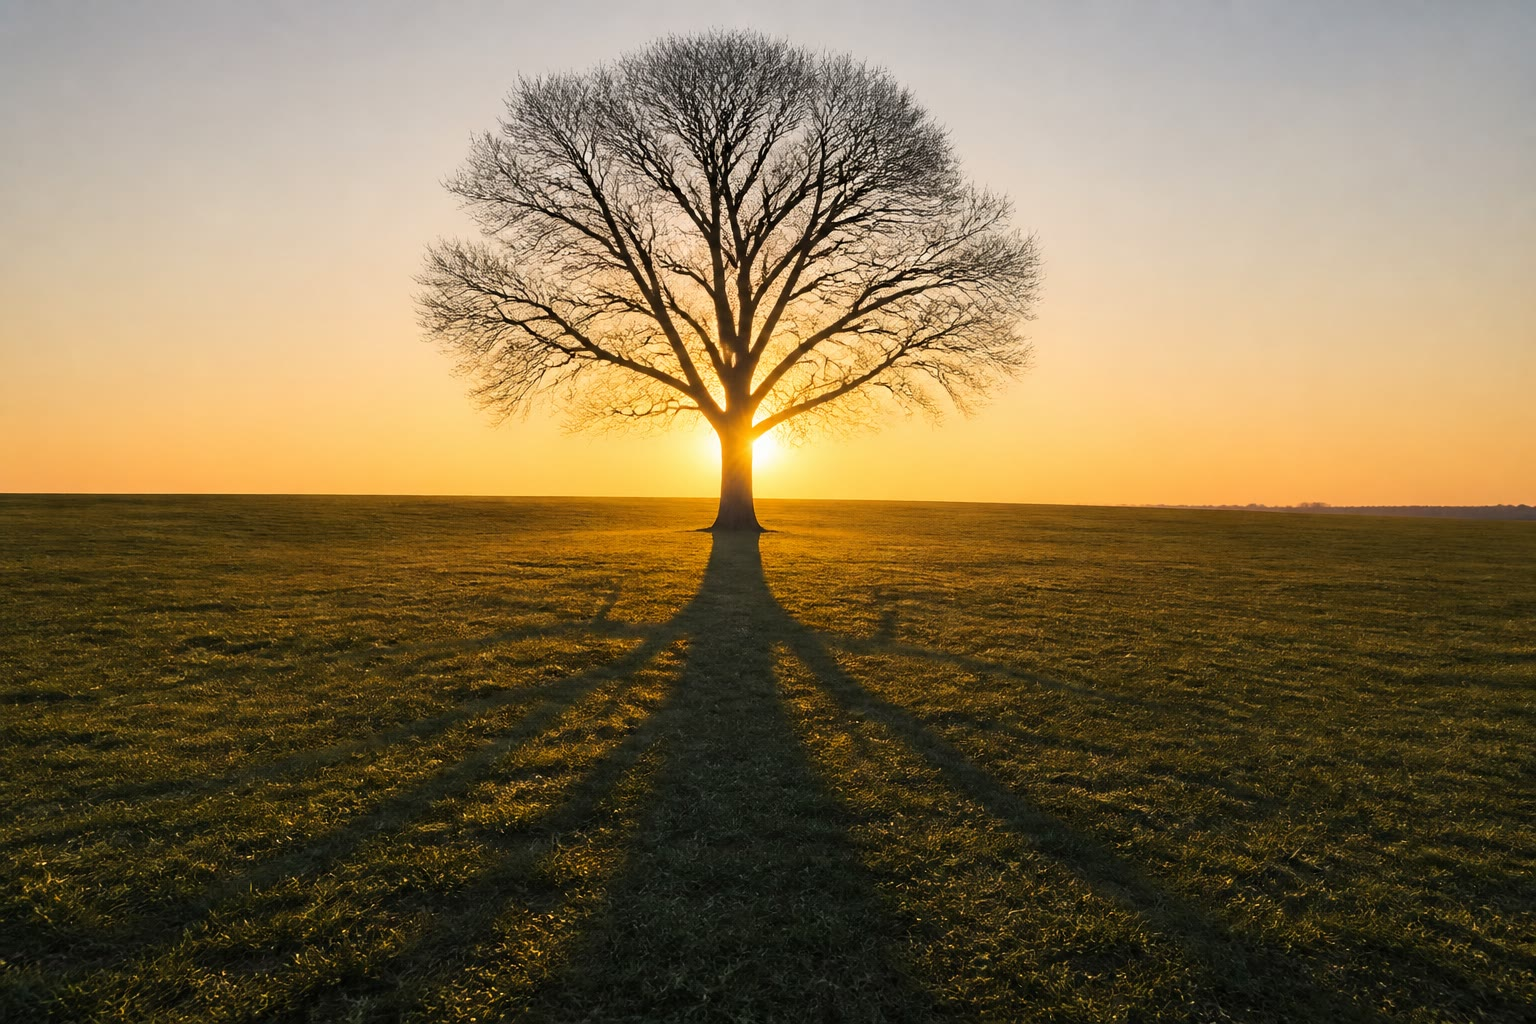
\includegraphics[width=0.6\linewidth]{images/book1/ai/g1-light-shadows-long-shadow.jpg}

{\small Een lage avondzon, een lange \omterm{def:g1:light-and-shadows:shadow}{schaduw}: hoe lager de Zon hangt, hoe verder elke \omterm{def:g1:light-and-shadows:shadow}{schaduw} zich uitstrekt.}
\end{omfigure}

\begin{example}[Probeer het: krijt om een schaduw]\label{ex:g1:light-and-shadows:chalk}
Sta op een zonnige ochtend stil op het schoolplein terwijl een vriend
met krijt een lijn om je \omterm{def:g1:light-and-shadows:shadow}{schaduw} trekt. Kom na de lunch terug en ga
op dezelfde plek staan: je \omterm{def:g1:light-and-shadows:shadow}{schaduw} is uit zijn krijtlijn gelopen en
van lengte veranderd! De Zon heeft haar plaats aan de hemel gewisseld
--- en de \omterm{def:g1:light-and-shadows:shadow}{schaduw} volgde. Het volgende hoofdstuk volgt de Zon een
hele dag lang.
\end{example}

\section{Oefeningen}

\begin{exercise}[$\star$]\label{exo:g1:light-and-shadows:1}
Sorteer in lichtbronnen en niet-bronnen: een kaarsvlam; \ de Maan;
\ een glimworm; \ een spiegel; \ een zaklamp; \ een witte muur.
\end{exercise}

\begin{exercise}[$\star$]\label{exo:g1:light-and-shadows:2}
Waarom zie je helemaal niets in een gesloten kamer zonder raam en
zonder lamp? Wat ontbreekt er?
\end{exercise}

\begin{exercise}[$\star$]\label{exo:g1:light-and-shadows:3}
Noem de drie dingen die je nodig hebt om een \omterm{def:g1:light-and-shadows:shadow}{schaduw} op de muur te
maken, en zet ze in de goede volgorde op een lijn.
\end{exercise}

\begin{exercise}[$\star$]\label{exo:g1:light-and-shadows:4}
De Zon staat links van je. Aan welke kant ligt je \omterm{def:g1:light-and-shadows:shadow}{schaduw}? Je draait
je helemaal om --- waar ligt hij nu?
\end{exercise}

\begin{exercise}[$\star$]\label{exo:g1:light-and-shadows:5}
Maak met \cref{met:g1:light-and-shadows:make} de \omterm{def:g1:light-and-shadows:shadow}{schaduw} van hetzelfde
stuk speelgoed eerst reusachtig en daarna klein. Wat heb je verschoven,
en welke kant op?
\end{exercise}

\begin{exercise}[$\star$]\label{exo:g1:light-and-shadows:6}
Kun je een \omterm{def:g1:light-and-shadows:shadow}{schaduw} oppakken en in je zak stoppen? Leg met
\cref{rem:g1:light-and-shadows:notathing} uit wat een \omterm{def:g1:light-and-shadows:shadow}{schaduw} echt is.
\end{exercise}

\begin{exercise}[$\star$]\label{exo:g1:light-and-shadows:7}
Waarom mag je nooit recht in de Zon kijken, terwijl je van het kijken
naar een lamp alleen maar een beetje verblind raakt?
\end{exercise}

\begin{exercise}[$\star$]\label{exo:g1:light-and-shadows:8}
Rond het middaguur hangt de Zon hoog; laat in de middag hangt ze
laag. Wanneer is je \omterm{def:g1:light-and-shadows:shadow}{schaduw} langer? Teken de twee \omterm{def:g1:light-and-shadows:shadow}{schaduwen} van een
boom, één voor elk moment.
\end{exercise}

\begin{exercise}[$\star\star$]\label{exo:g1:light-and-shadows:9}
Mia zegt: ``Mijn \omterm{def:g1:light-and-shadows:shadow}{schaduw} lag voor me, en nadat ik me omdraaide lag hij
achter me --- dus de \omterm{def:g1:light-and-shadows:shadow}{schaduw} draaide met mij mee.'' Sam zegt dat de
\omterm{def:g1:light-and-shadows:shadow}{schaduw} helemaal niet is bewogen. Denk aan
\cref{ex:g1:light-and-shadows:opposite}: wie heeft gelijk, en waarom
\emph{leek} het alsof de \omterm{def:g1:light-and-shadows:shadow}{schaduw} meedraaide?
\end{exercise}
